\documentclass{article}
\usepackage{tikz}
\usepackage{float} 
\usepackage{algorithm}
\usepackage{algpseudocode}
\usepackage{amsmath}
\usepackage{amssymb}
\usepackage{amsthm}
\usepackage{placeins}

% Define the 'definition' environment
\newtheorem{definition}{Definition}

\title{Segment Trees in Algorithmic Problems}
\author{Piotr Szczepaniak}
\date{\today}

\begin{document}

\maketitle

\tableofcontents

\begin{abstract}
This document provides an overview of segment trees. In the first place
I will describe some algebraic topics which are necessary for better
understanding how and why segment trees works. This knowledge will be useful
for reading the rest of the paper where We will dive into different kinds of trees.
For each structure, I will explain how it work and how to apply it to problems.
Then, I will look at each structure's time complexity and space complexity.
\end{abstract}

\section{Foundations of Segment Trees}
A segment tree is a binary tree used for storing information about segments. 
To efficently retrieve or update informations about elements stored 
in segment tree we can perform various operations most common of which are
query/update on point or range.
One of the examples can be maximum value of 
elements in given range or sum of elements in given range.

\begin{figure}[H]
    \centering
    
\begin{center}
    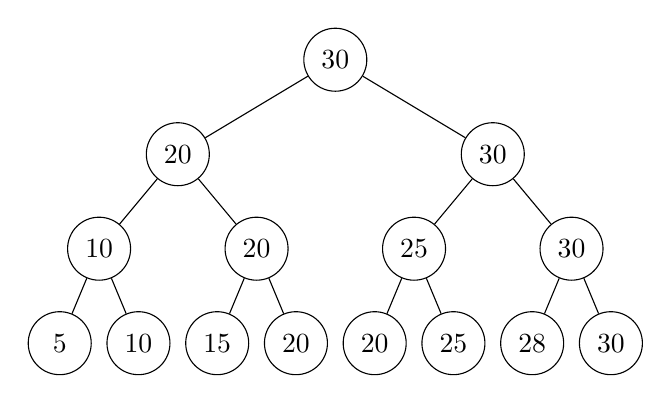
\begin{tikzpicture}[
      level distance=1.2cm,
      level 1/.style={sibling distance=4cm},
      level 2/.style={sibling distance=2cm},
      level 3/.style={sibling distance=1cm},
      every node/.style={draw,circle,minimum size=8mm,inner sep=1pt}
    ]
    
    % Root node with max value
    \node {30}
        child {node {20}
            child {node {10}
                child {node {5}}
                child {node {10}}
            }
            child {node {20}
                child {node {15}}
                child {node {20}}
            }
        }
        child {node {30}
            child {node {25}
                child {node {20}}
                child {node {25}}
            }
            child {node {30}
                child {node {28}}
                child {node {30}}
            }
        };
    
    \end{tikzpicture}
\end{center}
    \caption{Example of a segment tree with maximum value of elements in given range.}
    \label{fig:segment_tree_1}
\end{figure}

\subsection{Segment Tree with point update and range query}
To ilustrate use case of segment tree we will construct tree with max value on segment.
Let's say we are given an array \(A = [5, 10, 15, 20, 30, 25, 28, 20]\) of length \(n = 8\).
For now let's assume that the input array is of size \(n = 2^{k}\) where \(k\) is integer (for different
sizes of input we will fill input array with neutral elements (see section 2) to make it's length a power of 2).
The height of tree is \(h = \log_2{n}\). Let's define \(dep(i)\) as depth of node i in our tree.
We can see that \(dep(root) = 0\) and \(dep(leaf) = h\).
We want to be able to perform the following operations:
\begin{itemize}
    \item \textbf{Build structure} \\
    We will create a segment tree from an array.
    To build a segment tree, we need to create a binary tree where each node will store the maximum value of elements in its subtree. \\
    \begin{algorithm}
    \caption{Build Segment Tree for Maximum on Segment (Iterative)}
    \begin{algorithmic}
        \Procedure{BuildTree}{arr, seg}
            \For{$i = 0$ \textbf{to} $n - 1$} \Comment{Fill leaves of the segment tree}
                \State $seg[n + i] \gets A[i]$
            \EndFor
            \For{$i = n - 1$ \textbf{downto} $1$} \Comment{Calculates nodes from bottom to top}
                \State $seg[i] \gets \max(seg[2 \times i], seg[2 \times i + 1])$
            \EndFor
        \EndProcedure
    \end{algorithmic}
\end{algorithm}

    \item \textbf{Point update} \\
    Now let's update single value in the array and update the tree.
    We will change the value of \(A[1]\) from 10 to 35.
    To update the tree we need to change the value of the leaf node 
    and then update all the parent nodes up to the root.
    \begin{algorithm}
    \caption{Point Update on Segment Tree }
    \begin{algorithmic}
        \Procedure{update}{seg, index, value}
            \State $index \gets index + n$ \Comment{Shift index to leaf}
            \State $arr[index] \gets value$ \Comment{Update the value at the leaf}
            \While{$index > 1$} \Comment{Update the parent nodes}
                \State $index \gets \lfloor index / 2 \rfloor$
                \State $arr[index] \gets \max(arr[2 \times index], arr[2 \times index + 1])$
            \EndWhile
        \EndProcedure
    \end{algorithmic}
\end{algorithm}
    \begin{figure}[H]
        \centering
        
\begin{center}
    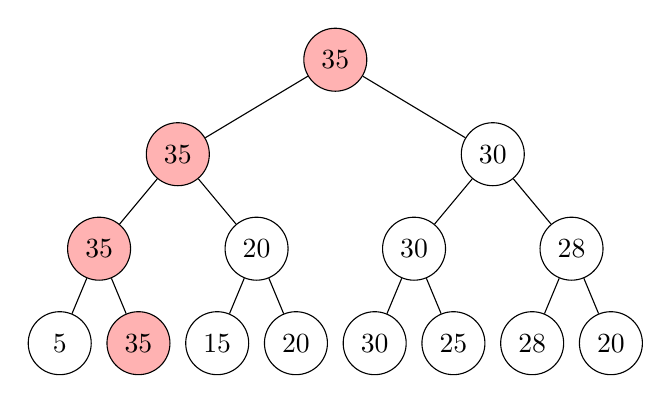
\begin{tikzpicture}[
      level distance=1.2cm,
      level 1/.style={sibling distance=4cm},
      level 2/.style={sibling distance=2cm},
      level 3/.style={sibling distance=1cm},
      every node/.style={draw,circle,minimum size=8mm,inner sep=1pt}
    ]
    
    % Root node with max value
    \node[fill=red!30] {35}
        child {node[fill=red!30] {35}
            child {node[fill=red!30] {35}
                child {node {5}}
                child {node[fill=red!30] {35}}
            }
            child {node {20}
                child {node {15}}
                child {node {20}}
            }
        }
        child {node {30}
            child {node {30}
                child {node {30}}
                child {node {25}}
            }
            child {node {28}
                child {node {28}}
                child {node {20}}
            }
        };
    
    \end{tikzpicture}
\end{center}

        \caption{Example of point update.}
        \label{fig:segment_tree_2}
    \end{figure}

    \item \textbf{Range query} \\
    Now let's say we want to find the maximum value in the range \(A[2:7]\).
    To do this we need to traverse the tree from the root to the leaves and 
    find nodes that are in the range. Then we will get max the values of these nodes to get the final result.
    To get the result for range \(A[2:7]\) we call \(RangeQuery(seg, 1, 1, 8, 2, 7)\).

    \begin{algorithm}
    \caption{Range Maximum Query on Segment Tree (Recursive, Close-Open Range)}
    \begin{algorithmic}[1]
        \Procedure{RangeQuery}{seg, index, l, r, a, b}
            \Comment{index: current node index in seg}
            \Comment{[l, r): segment represented by current node}
            \Comment{[a, b): query range}
            \If{$b \le l$ \textbf{or} $r \le a$}
                \State \Return $-\infty$ \Comment{No overlap}
            \ElsIf{$a \le l$ \textbf{and} $r \le b$}
                \State \Return $seg[index]$ \Comment{Total overlap}
            \Else
                \State $mid \gets \left\lfloor \frac{l + r}{2} \right\rfloor$
                \State $left \gets$ \Call{RangeQuery}{seg, $2 \cdot index$, $l$, $mid$, $a$, $b$}
                \State $right \gets$ \Call{RangeQuery}{seg, $2 \cdot index + 1$, $mid$, $r$, $a$, $b$}
                \State \Return $\max(left, right)$
            \EndIf
        \EndProcedure
    \end{algorithmic}
\end{algorithm}

    \begin{figure}[H]
        \centering
        
\begin{center}
    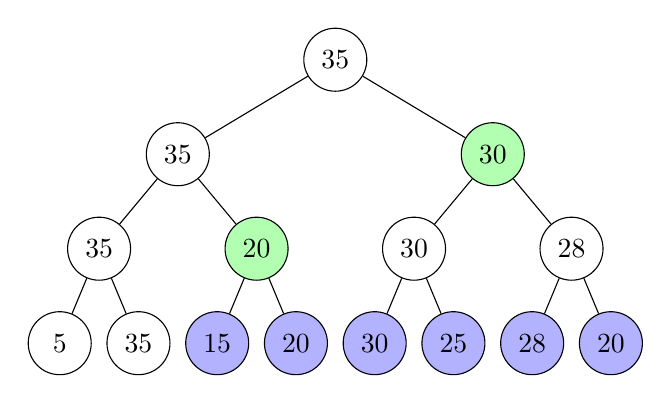
\begin{tikzpicture}[
      level distance=1.2cm,
      level 1/.style={sibling distance=4cm},
      level 2/.style={sibling distance=2cm},
      level 3/.style={sibling distance=1cm},
      every node/.style={draw,circle,minimum size=8mm,inner sep=1pt}
    ]
    
    % Root node with max value
    \node {35}
        child {node {35}
            child {node {35}
                child {node {5}}
                child {node {35}}
            }
            child {node[fill=green!30] {20}
                child {node[fill=blue!30]  {15}}
                child {node[fill=blue!30]  {20}}
            }
        }
        child {node[fill=green!30]  {30}
            child {node {30}
                child {node[fill=blue!30]  {30}}
                child {node[fill=blue!30]  {25}}
            }
            child {node  {28}
                child {node[fill=blue!30]  {28}}
                child {node[fill=blue!30] {20}}
            }
        };
    
    \end{tikzpicture}
\end{center}

        \caption{Example of range query. Blue leafs represents subarray \(A[2:7]\). Green nodes 
        represents nodes where ranges totally overlap and we can get max value. The result of the query is 30.}
        \label{fig:segment_tree_3}
    \end{figure}

\end{itemize}

\subsection{Segment Tree with range update and range query}
A Little more complex version of segment tree is a segment tree with range update and range query which require \textbf{lazy propagation}.
We will consider a segment tree with sum of elements in given range. 
Apart form values in tree we will also store lazy values in each node.
The lazy value is used to delay the update of a node until it is needed.
\begin{itemize}
    \item \textbf{Build structure} 
    Only difference form previus example is initializig the lazy value for all nodes \\
    \begin{algorithm}
    \caption{Build Segment Tree for Sum on Segment (Iterative)}
    \begin{algorithmic}
        \Procedure{BuildTree}{arr, seg}
            \For{$i = 0$ \textbf{to} $n - 1$} \Comment{Fill leaves of the segment tree}
                \State $seg[n + i] \gets \{A[i], 0\}$ \Comment{second value is for lazy propagation}
            \EndFor
            \For{$i = n - 1$ \textbf{downto} $1$} \Comment{Calculates nodes from bottom to top}
                \State $seg[i] \gets \{\max(seg[2 \times i], seg[2 \times i + 1]), 0\}$
            \EndFor
        \EndProcedure
    \end{algorithmic}
\end{algorithm}\\


    \item \textbf{Range update} \\
    In this case lazy value is a value that we want to add to all elements in the range.
    Another way to think about this is that we want to add lazy value to all elenets in arrary 
    which are represented by all leaves in subtree of given node.
    \begin{algorithm}
    \caption{Range Update on Segment Tree }
    \begin{algorithmic}
        \Procedure{QueryUpdate}{seg, lazy index, l, r, a, b, value} \Comment{Value: value we wanted to add to each element in array}
            \State $size = r - l + 1$
            \If{$b < l$ \textbf{or} $a > r$}
                \State \Return
            \ElsIf{$a \leq l$ \textbf{and} $r \leq b$}
                \State $seg[index] \gets {seg[index] + value*size}$
                \State $lazy[index] \gets {lazy[index] + value}$
                \State \Return
            \Else
                \State $seg[index*2] \gets {seg[index*2] + value*size}$ \Comment{Update left child}
                \State $lazy[index*2] \gets {lazy[index*2] + value}$ \Comment{Push lazy to left child}
                \State $seg[index*2+1] \gets {seg[index*2+1] + value*size}$ \Comment{Same to right}
                \State $lazy[index*2+1] \gets {lazy[index*2+1] + value}$ 
                \State $lazy[index] \gets {0}$ \Comment{Reset lazy value for current node}
                \State $mid \gets \left\lfloor \frac{l + r}{2} \right\rfloor$
                \State $left \gets$ \Call{QueryUpdate}{seg, $2 \cdot index$, $l$, $mid$, $a$, $b$, $value$}
                \State $right \gets$ \Call{QueryUpdate}{seg, $2 \cdot index + 1$, $mid + 1$, $r$, $a$, $b$, $value$}
                \State $seg[index] \gets {seg[index*2] + seg[index*2+1] + lazy[index]*size}$ \Comment{Update current node after lazy propagation}
            \EndIf
        \EndProcedure
    \end{algorithmic}
\end{algorithm} \\
    How this algorithm works:
    \begin{enumerate}
        \item If the current node is fully in range update the sum of the node and set the lazy value. Sum - $value*size$ where $size$ is the number of array elements (leafs) in the range of this node, Lazy is equal to $value$, which we will later push down to child nodes.
        \item If not fully in range push the lazy value down to the child nodes and update their sum and also reset the lazy value for the current node.
        \item Call the function recursively for the left and right child nodes.
        \item Finally update the sum of the current node with the sum of its children.
    \end{enumerate}
    On the following example we will update the range \(A[0:5]\) by adding 10 to all elements in this range
    where initial array is \(A = [5, 10, 15, 20, 30, 25, 20, 20]\).
    
    \begin{figure}[H]
        \centering
        
\begin{center}
    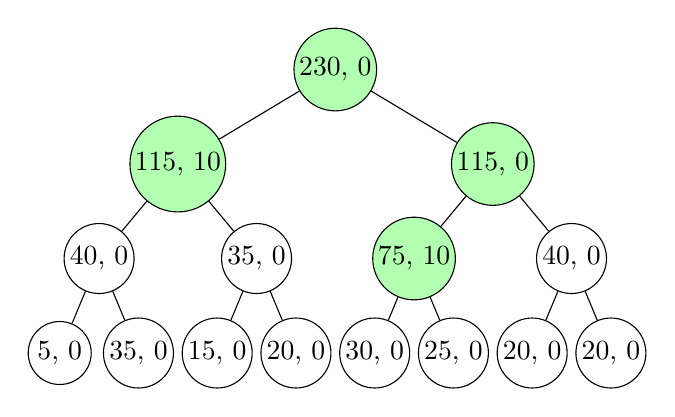
\begin{tikzpicture}[
      level distance=1.2cm,
      level 1/.style={sibling distance=4cm},
      level 2/.style={sibling distance=2cm},
      level 3/.style={sibling distance=1cm},
      every node/.style={draw,circle,minimum size=8mm,inner sep=1pt}
    ]
    
    % Root node with max value
    \node[fill=green!30] {230, 0}
        child {node[fill=green!30] {115, 10}
            child {node {40, 0}
                child {node {5, 0}}
                child {node {35, 0}}
            }
            child {node {35, 0}
                child {node  {15, 0}}
                child {node {20, 0}}
            }
        }
        child {node[fill=green!30] {115, 0}
            child {node[fill=green!30] {75, 10}
                child {node {30, 0}}
                child {node {25, 0}}
            }
            child {node  {40, 0}
                child {node {20, 0}}
                child {node {20, 0}}
            }
        };
    
    \end{tikzpicture}
\end{center}

        \caption{This is state of the tree after range update. Green nodes were changed during the update.}
        \label{fig:segment_tree_4}
    \end{figure}

    \item \textbf{Range query} 
    We will try to retrieve the sum of some given range. The algorithm for this will be simiar to the one for range update.
    First we will check if the current node is fully in range. If it is we add the sum of this node, propagating lazy values along the way.
    \begin{algorithm}[H]
    \caption{Range Query on Segment Tree for Max with Modifiers}
    \begin{algorithmic}
        \Procedure{RangeQuery}{seg, index, l, r, a, b}
            \If{$b \leq l$ \textbf{or} $r \leq a$}
                \State \Return $-\infty$
            \EndIf
            \If{$a \leq l$ \textbf{and} $r \leq b$}
                \State \Return $seg[index].val$
            \EndIf
            \State $mid \gets \left\lfloor \frac{l + r}{2} \right\rfloor$
            \State $left \gets$ \Call{RangeQuery}{seg, $2 \cdot index$, $l$, $mid$, $a$, $b$}
            \State $right \gets$ \Call{RangeQuery}{seg, $2 \cdot index + 1$, $mid$, $r$, $a$, $b$}
            \State \Return $\max(left, right) + seg[index].mod$
        \EndProcedure
    \end{algorithmic}
\end{algorithm}
 
    
    \begin{figure}[H]
        \centering
        
\begin{center}
    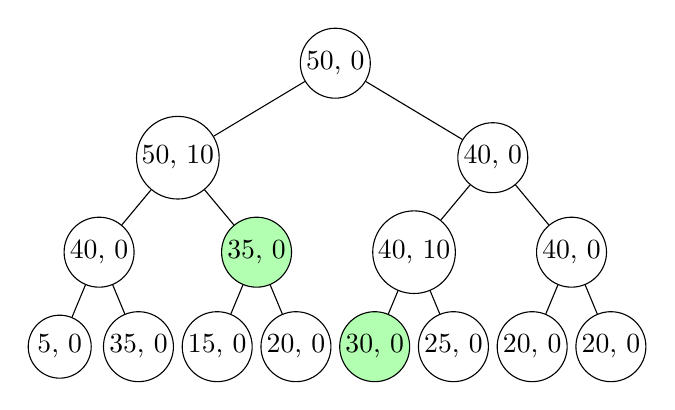
\begin{tikzpicture}[
      level distance=1.2cm,
      level 1/.style={sibling distance=4cm},
      level 2/.style={sibling distance=2cm},
      level 3/.style={sibling distance=1cm},
      every node/.style={draw,circle,minimum size=8mm,inner sep=1pt}
    ]
    
    % Root node with max value
    \node {50, 0}
        child {node {50, 10}
            child {node {40, 0}
                child {node {5, 0}}
                child {node {35, 0}}
            }
            child {node [fill=green!30] {35, 0}
                child {node  {15, 0}}
                child {node {20, 0}}
            }
        }
        child {node {40, 0}
            child {node {40, 10}
                child {node [fill=green!30] {30, 0}}
                child {node {25, 0}}
            }
            child {node  {40, 0}
                child {node {20, 0}}
                child {node {20, 0}}
            }
        };
    
    \end{tikzpicture}
\end{center}

        \caption{This is state of the tree after range query on range [2: 4]. Green nodes were we took values form to the sum. Result of query is 95.}
        \label{fig:segment_tree_5}
    \end{figure}

\end{itemize}


\section{A mathematical approach to segment trees}
In this section we will try to understand how segment trees work and why they are so efficient.
In order to do this we will need to understand some basic algebra that is used in segment trees.


\subsection{Monoids}
A monoid \( (S, \ast, e) \) is a set equipped with an associative binary operation \( S \times S \to S \) and
an identity element \(e\). 
\begin{itemize}
    \item \textbf{Associativity} \\
    For all \( a, b, c \in S \), \( (a \ast b) \ast c = a \ast (b \ast c) \).
    \item \textbf{Identity element} \\
    There exists an element \( e \in S \) such that for all \( a \in S \), \( a \ast e = e \ast a = a \).
    \item \textbf{Commutativity} \\
    Monoid is called \textbf{commutative} if for all \( a, b \in S \), \( a \ast b = b \ast a \).
\end{itemize}
Examples of monoids:
\begin{itemize}
    \item \textbf{Natural numbers under addition, (\(\mathbb{N}\), +, 0) } \\
    In this simple example we can see that addition is associative and commutative. 
    Adding 0 (neutral element) to any of the numbers will not change the result of the operation.
    \item \textbf{Strings over an alphabet, (\(\Sigma^*\), \(\cdot\), \(\epsilon\))} \\
    \(\Sigma^*\) - set of all strings over an alphabet \(\Sigma\) \\
    \(\cdot\) - concatenation of strings \\
    \(\epsilon\) - empty string \\
    This is a example of non-commutative monoid. Concatenation of strings is associative but not commutative as we can see in the following example.
    \begin{equation}
        \text{abc} \cdot \text{def} = \text{abcdef} \neq \text{defabc} = \text{def} \cdot \text{abc}
    \end{equation}
\end{itemize}
\subsection{Homomorphism}
A homomorphism is a structure-preserving map between two algebraic structures.
In this section we will look at homomorphisms between monoids.
Let \( (S, \ast, e) \) and \( (T, \cdot, \theta) \) be two monoids.
A function \( f: S \to T \) is a homomorphism if:
\begin{itemize}
    \item \textbf{Preserves the operation} \\
    For all \( a, b \in S \), \( f(a \ast b) = f(a) \cdot f(b) \).
    \item \textbf{Preserves the identity element} \\
    \( f(e) = \theta \).
\end{itemize}
Let's consider a simple example of homomorphism between two monoids.
Let \( S = (\mathbb{N}, +, 0) \) and \( T = (\mathbb{N}, \cdot, 1) \).
Let \( f: S \to T \) be defined as \( f(x) = 2^x \).
We can see that:
\begin{itemize}
    \item \( f(a + b) = 2^{a + b} = 2^a \cdot 2^b = f(a) \cdot f(b) \)
    \item \( f(0) = 2^0 = 1 \)
\end{itemize}
\subsection{Endomorphism}
A special case of homomorphism is an endomorphism.
This is a homomorphism from a monoid to itself.
Lets consider a simple example of endomorphism.
Let \( S = (\mathbb{N}, +, 0) \) and \( f: S \to S \) be defined as \( f(x) = x + 1 \).
We can see that:
\begin{itemize}
    \item \( f(a + b) = a + b + 1 = (a + 1) + (b + 1) = f(a) + f(b) \)
    \item \( f(0) = 0 + 1 = 1 \)
\end{itemize}
Interesing property of endomorphisms is that a Set of all endomorphisms of a monoid is also a monoid.
Let's consider a set of all endomorphisms of a monoid \( S \).
Let \( S = (\mathbb{N}, +, 0) \) and let \( E \) be a set of all endomorphisms of \( S \).
We can define a binary operation on \( E \) as follows:
\begin{equation}
    f \ast g = h \text{ where } h(x) = f(g(x))
\end{equation}
We can see that this operation is associative and has an identity element \( e(x) = x \).

\subsection{Application of Monoids to Segment Trees}
How does this all relate to segment trees?
First of all we can see that segment trees requires the properties of monoids to work.
The associativity of the operation is required to be able to combine the results of the operations on the segments.
The identity element is required when we ask for the result of the operation on an empty segment or 
when we want extend our initial array to a power of 2. 
Since all segment trees must preserve monoid properties, we can think more generic 
approach to the implementation. We will try to create a generic segment tree that can be used for any monoid for 
range queries and point updates. Let \(\ast\) be a binary operation on a monoid \(S\) and let \(e\) be the identity element of the monoid.

\begin{algorithm}
    \caption{Segment Tree over a Monoid \((S, \ast, e)\)}
    \begin{algorithmic}[1]
        \Procedure{BuildTree}{$A$, $seg$, $e$}
            \State $n \gets$ next power of two greater than or equal to $|A|$
            \For{$i = 0$ \textbf{to} $|A| - 1$}
                \State $seg[n + i] \gets A[i]$ \Comment{Insert original values}
            \EndFor
            \For{$i = |A|$ \textbf{to} $n - 1$}
                \State $seg[n + i] \gets e$ \Comment{Pad remaining leaves with identity}
            \EndFor
            \For{$i = n - 1$ \textbf{downto} $1$}
                \State $seg[i] \gets seg[2 \times i] \ast seg[2 \times i + 1]$
            \EndFor
        \EndProcedure

        \\
        
        \Procedure{Update}{$arr$, $index$, $value$}
            \State $index \gets index + n$ \Comment{Move to the leaf node}
            \State $arr[index] \gets value$ \Comment{Set the new value at the leaf}
            \While{$index > 1$}
                \State $index \gets \lfloor index / 2 \rfloor$ \Comment{Move to parent}
                \State $arr[index] \gets arr[2 \times index] \ast arr[2 \times index + 1]$
            \EndWhile
        \EndProcedure

        \\

        \Procedure{RangeQuery}{$seg$, $index$, $l$, $r$, $a$, $b$, $e$}
        \Comment{$index$: current node in segment tree}
        \Comment{$[l, r]$: range covered by node}
        \Comment{$[a, b]$: query range}
        \If{$b \leq l$ \textbf{or} $r \leq a$}
            \State \Return $e$ \Comment{No overlap}
        \ElsIf{$a \leq l$ \textbf{and} $r \leq b$}
            \State \Return $seg[index]$ \Comment{Total overlap}
        \Else
            \State $mid \gets \left\lfloor \frac{l + r}{2} \right\rfloor$
            \State $left \gets$ \Call{RangeQuery}{$seg$, $2 \cdot index$, $l$, $mid$, $a$, $b$, $e$}
            \State $right \gets$ \Call{RangeQuery}{$seg$, $2 \cdot index + 1$, $mid$, $r$, $a$, $b$, $e$}
            \State \Return $left \ast right$
        \EndIf
    \EndProcedure
    \end{algorithmic}
\end{algorithm}
\vspace{0.1cm}
\begin{algorithm}
    \caption{Generic Point Update in a Segment Tree over a Monoid \((S, \ast, e)\)}
    \begin{algorithmic}[1]
        \Procedure{Update}{$arr$, $index$, $value$}
            \State $index \gets index + n$ \Comment{Move to the leaf node}
            \State $arr[index] \gets value$ \Comment{Set the new value at the leaf}
            \While{$index > 1$}
                \State $index \gets \lfloor index / 2 \rfloor$ \Comment{Move to parent}
                \State $arr[index] \gets arr[2 \times index] \ast arr[2 \times index + 1]$
            \EndWhile
        \EndProcedure
    \end{algorithmic}
\end{algorithm} 
\vspace{0.1cm}
\begin{algorithm}
    \caption{Range Query on Segment Tree over Monoid \((S, \ast, e)\)}
    \begin{algorithmic}[1]
        \Procedure{RangeQuery}{$seg$, $index$, $l$, $r$, $a$, $b$, $e$}
            \Comment{$index$: current node in segment tree}
            \Comment{$[l, r]$: range covered by node}
            \Comment{$[a, b]$: query range}
            \If{$b < l$ \textbf{or} $a > r$}
                \State \Return $e$ \Comment{No overlap}
            \ElsIf{$a \leq l$ \textbf{and} $r \leq b$}
                \State \Return $seg[index]$ \Comment{Total overlap}
            \Else
                \State $mid \gets \left\lfloor \frac{l + r}{2} \right\rfloor$
                \State $left \gets$ \Call{RangeQuery}{$seg$, $2 \cdot index$, $l$, $mid$, $a$, $b$, $e$}
                \State $right \gets$ \Call{RangeQuery}{$seg$, $2 \cdot index + 1$, $mid + 1$, $r$, $a$, $b$, $e$}
                \State \Return $left \ast right$
            \EndIf
        \EndProcedure
    \end{algorithmic}
\end{algorithm} 
\FloatBarrier
Now we can replace this generic monoid with some specific one.
For example we can use a segment tree for sum of elements in given range.
In this case we will use \(\ast\) as addition and \(e\) as 0. 
Another example can be a segment tree for maximum value in given range.
In this case we will use \(\ast\) as maximum and \(e\) as \(-\infty\).
We can see that using this generic approach we can create a segment tree for any monoid.

\subsection{Application of Endomorphisms to Segment Trees}
In this section we will try to implement a generic segment tree for range update and range query.
In order to do this we will need to use endomorphisms and their properties.
Let's consider what happens when we update a range of elements in the segment tree.
What we acctually do is application of endomorphism on some range of elements. This operation
doesn't break the structure of the segment tree, because endomorphism is a function that doesn't change the structure of the monoid.
Making multiple updates (that is applying multiple endomorphisms) on the same range of elements 
also doesn't break the structure of the segment tree.
This statement follows form the fact which we showed erlier that the set of all endomorphisms of a monoid is also a monoid.
Multiple updates are just composition of endomorphisms.
Let's consider a simple example: \\
We have a segment tree that can add some value to a range of elements and query the sum of elements in a range.
Let's say we updated some range of elements by adding 1 to them,
we can look at this as applying an endomorphism \(f_1(x) = x + 1\) to the range of elements.
We also updated the same range of elements by adding 5 to them, (again endomorphism \(f_5(x) = x + 5\)).
In result we apply composition of both endomorphisms to the range of elements.
The result of this operation is the same as applying endomorphism \(f_6(x) = x + 6\) to the range of elements.
We can see that composition of endomorphisms is also an endomorphism (endomorphisms are monoid).
Now we will try to implement a generic segment tree for range update and range query.
Let \(\ast\) be a binary operation on a monoid \(S\) and let \(e\) be the identity element of the monoid.
Let \(e(x) = x\) be a identity element for monoid of endomorphisms
\begin{algorithm}[H]
    \caption{Range Update on Segment Tree over value Monoid and modifier Monoid }
    \begin{algorithmic}[1]
        \Procedure{RangeUpdate}{seg, index, l, r, a, b, $f$}
            \If{$b \le l$ \textbf{or} $r \le a$}
                \State \Return
            \ElsIf{$a \le l$ \textbf{and} $r \le b$}
                \State $seg[index].val \gets f(seg[index].val)$
                \State $seg[index].mod \gets f \circ seg[index].mod$ \Comment{Keep in mind the order of operations}
                \State \Return
            \Else
                \State $mid \gets \lfloor (l + r)/2 \rfloor$
                \State \Call{RangeUpdate}{seg, $2 \cdot index$, $l$, $mid$, $a$, $b$, f}
                \State \Call{RangeUpdate}{seg, $2 \cdot index + 1$, $mid$, $r$, $a$, $b$, f}
                \State \Call{Pull}{seg, index}
            \EndIf
        \EndProcedure

        \\

        \Procedure{RangeQuery}{seg, index, l, r, a, b}
            \If{$b \le l$ \textbf{or} $r \le a$}
                \State \Return $e$
            \ElsIf{$a \le l$ \textbf{and} $r \le b$}
                \State \Return $seg[index].val$
            \Else
                \State $mid \gets \lfloor (l + r)/2 \rfloor$
                \State $left \gets$ \Call{RangeQuery}{seg, $2 \cdot index$, $l$, $mid$, $a$, $b$}
                \State $right \gets$ \Call{RangeQuery}{seg, $2 \cdot index + 1$, $mid$, $r$, $a$, $b$}
                \State \Return $f(left \oplus right)$ 
            \EndIf
        \EndProcedure

        \\

        \Procedure{Pull}{seg, index}
            \State $seg[index].val \gets seg[index].mod\big(seg[2 \cdot index].val \oplus seg[2 \cdot index + 1].val\big)$
        \EndProcedure


    \\

    \Procedure{Push}{seg, index}
        \State $seg[2 \cdot index].val \gets seg[index].mod(seg[2 \cdot index].val) $
        \State $seg[2 \cdot index].mod \gets  seg[index].mod \circ seg[2 \cdot index].mod$
        \State $seg[2 \cdot index + 1].val \gets  seg[index].mod(seg[2 \cdot index + 1].val) $
        \State $seg[2 \cdot index + 1].mod \gets  seg[index].mod \circ seg[2 \cdot index + 1].mod$
        \State $seg[2 \cdot index].mod \gets id$ \Comment{Reset the modifier}
    \EndProcedure
    \end{algorithmic}
\end{algorithm}

\vspace{0.1cm}
\begin{algorithm}
    \caption{Range Update on Segment Tree over Monoid \((S, \ast, e)\)}
    \begin{algorithmic}[1]
        \Procedure{RangeUpdate}{$seg$, $lazy$, $index$, $l$, $r$, $a$, $b$, $value$, $e$}
            \State \textbf{Call:} \textsc{PushDown}(index, l, r, lazy, e)
            \If{$b < l$ \textbf{or} $a > r$}
                \State \Return \Comment{No overlap, do nothing}
            \ElsIf{$a \leq l$ \textbf{and} $r \leq b$}
                \State $seg[index] \gets \ast(seg[index], (r - l + 1) \times value)$
                \State $lazy[index] \gets \ast(lazy[index], value)$
            \Else
                \State $mid \gets \left\lfloor \frac{l + r}{2} \right\rfloor$
                \State \textsc{RangeUpdate}(seg, lazy, 2 $\times$ index, l, mid, a, b, value, e)
                \State \textsc{RangeUpdate}(seg, lazy, $2 \times index + 1$, mid + 1, r, a, b, value, e)
                \State $seg[index] \gets \ast(seg[2 \times index], seg[2 \times index + 1])$
            \EndIf
        \EndProcedure

        \Procedure{PushDown}{$index$, $l$, $r$, $lazy$, $e$}
            \If{$lazy[index] \neq e$}
                \State $seg[index] \gets \ast(seg[index], lazy[index])$
                \If{$l \neq r$}
                    \State $lazy[2 \times index] \gets \ast(lazy[2 \times index], lazy[index])$
                    \State $lazy[2 \times index + 1] \gets \ast(lazy[2 \times index + 1], lazy[index])$
                \EndIf
                \State $lazy[index] \gets e$ \Comment{Clear lazy value after pushing it down}
            \EndIf
        \EndProcedure
    \end{algorithmic}
\end{algorithm}

\vspace{0.1cm}
\begin{algorithm}
    \caption{Range Query on Segment Tree over Monoid \((S, \ast, e)\)}
    \begin{algorithmic}[1]
        \Procedure{RangeQuery}{$seg$, $lazy$, $index$, $l$, $r$, $a$, $b$, $e$}
            \State \textbf{Call:} \textsc{PushDown}(index, l, r, lazy, e)
            \If{$b < l$ \textbf{or} $a > r$}
                \State \Return $e$ \Comment{No overlap, return identity element}
            \ElsIf{$a \leq l$ \textbf{and} $r \leq b$}
                \State \Return $seg[index]$ \Comment{Total overlap, return the current node's value}
            \Else
                \State $mid \gets \left\lfloor \frac{l + r}{2} \right\rfloor$
                \State $left \gets$ \Call{RangeQuery}{$seg$, $lazy$, $2 \times index$, $l$, $mid$, $a$, $b$, $e$}
                \State $right \gets$ \Call{RangeQuery}{$seg$, $lazy$, $2 \times index + 1$, $mid + 1$, $r$, $a$, $b$, $e$}
                \State \Return $\ast(left, right)$ \Comment{Combine results from left and right child using \(\ast\)}
            \EndIf
        \EndProcedure

        \Procedure{PushDown}{$index$, $l$, $r$, $lazy$, $e$}
            \If{$lazy[index] \neq e$}
                \State $seg[index] \gets \ast(seg[index], lazy[index])$
                \If{$l \neq r$}
                    \State $lazy[2 \times index] \gets \ast(lazy[2 \times index], lazy[index])$
                    \State $lazy[2 \times index + 1] \gets \ast(lazy[2 \times index + 1], lazy[index])$
                \EndIf
                \State $lazy[index] \gets e$ \Comment{Clear lazy value after pushing it down}
            \EndIf
        \EndProcedure
    \end{algorithmic}
\end{algorithm}
 
\FloatBarrier
Using this generic approach we can simply replace the monoid with some specific one and
set endomorphism as some function that we want to apply to the range of elements.

\section{Binsearch on Segment Tree}
In this section we will see that we can use segment trees not only for queries and updates but also for
binary search. Let's consider the following problem:
\begin{center}
    \textit{Given an array $a[1 \ldots n]$, answer a query $Q(i, j, x)$: What is the smallest index $k$ so that $a[k] \geq x$ in subarray  $a[i \ldots j]$?}\\[1ex]
\end{center}

We want to be able to answer this query in \(O(\log{n})\) time. We can create 
a segment tree with max value in given range but this is not enough. We need to upgrade our segment tree
with binsearch operation, which goes as follows:
\begin{itemize}
    \item Traverse recursively the tree to find the nodes that are in the range of the query (just like in range query). Always go to the left child first.
    \item For every nodes perform a binary search on the subtree.
    \item Binsearch 
        \begin{itemize}
            \item if right child's value is less than x, return -1 (no such index)
            \item if left child's value is greater than x, go to left child
            \item else go to right child
        \end{itemize}
    \item Because we traverse the tree from left to right, we can be sure that the first binsearch that returns index different than -1 is the answer to the query.
    \item if no such index was found, return -1.
\end{itemize}

\begin{algorithm}
    \caption{Find First Index With Value Greater Than $x$ in Range $[a, b)$}
    \begin{algorithmic}[1]
        \Procedure{Query}{segTree, index, l, r, a, b, x}
            \Comment{index: current node index}
            \Comment{[l, r): segment represented by current node}
            \Comment{[a, b): query range}
            \If{$b \leq l$ \textbf{or} $r \leq a$}
                \State \Return $-1$ \Comment{No overlap}
            \ElsIf{$a \leq l$ \textbf{and} $r \leq b$}
                \State \Return \Call{BinarySearch}{segTree, index, x}
            \Else
                \State $mid \gets \left\lfloor \frac{l + r}{2} \right\rfloor$
                \State $left \gets$ \Call{Query}{segTree, $2 \cdot index$, $l$, $mid$, $a$, $b$, $x$}
                \If{$left \neq -1$}
                    \State \Return $left$
                \EndIf
                \State \Return \Call{Query}{segTree, $2 \cdot index + 1$, $mid$, $r$, $a$, $b$, $x$}
            \EndIf
        \EndProcedure
        \\
        \Procedure{BinarySearch}{tree, index, x}
            \While{$index*2 < tree.size$}
                \State $left \gets tree[index * 2]$
                \If{$left > x$}
                    \State $index \gets index * 2$
                \Else
                    \State $index \gets index * 2 + 1$
                \EndIf
            \EndWhile
            \If{$tree[index] > x$}
                \State \Return $index$
            \Else
                \State \Return $-1$ \Comment{No index found}
            \EndIf
        \EndProcedure
    \end{algorithmic}
\end{algorithm}

\FloatBarrier
Let's consider the following example: \\
We have an array \(A = [5, 8, 2, 7, 1, 11, 13, 12, 19, 14, 15, 0, 15, 10, 15, 4]\) and we want to find the smallest index \(k\) such that \(A[k] \geq 14\) in the range \(A[5:12]\).

\begin{figure}[H]
    \centering
    
\begin{center}
    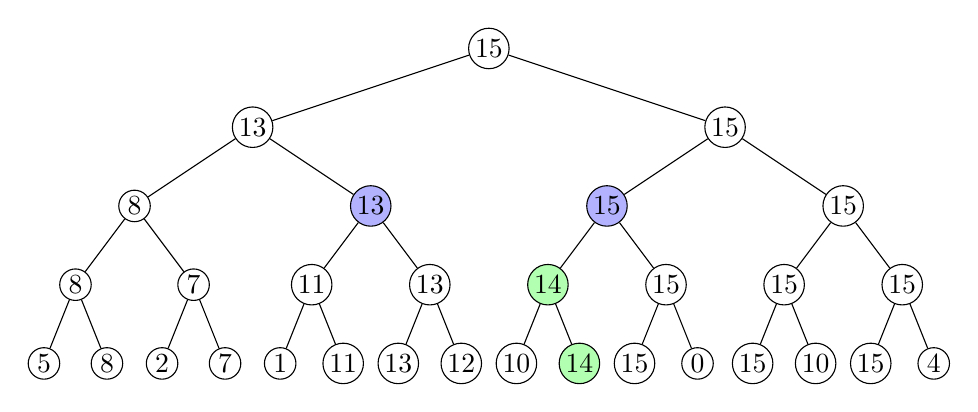
\begin{tikzpicture}[
        level distance=1cm,
        sibling distance=0pt,
        every node/.style = {circle, draw, minimum size=4mm, inner sep=1pt},
        level 1/.style={sibling distance=6cm},
        level 2/.style={sibling distance=3cm},
        level 3/.style={sibling distance=1.5cm},
        level 4/.style={sibling distance=0.8cm},
        level 5/.style={sibling distance=0.5cm}
      ]
      
      \node {15}
      child {node {13}
        child {node {8}
          child {node {8}
            child {node {5}}
            child {node {8}}
          }
          child {node {7}
            child {node {2}}
            child {node {7}}
          }
        }
        child {node[fill=blue!30] {13}
          child {node {11}
            child {node {1}}
            child {node {11}}
          }
          child {node {13}
            child {node {13}}
            child {node {12}}
          }
        }
      }
      child {node {15}
        child {node[fill=blue!30] {15}
          child {node[fill=green!30] {14}
            child {node {10}}
            child {node[fill=green!30] {14}}
          }
          child {node {15}
            child {node {15}}
            child {node {0}}
          }
        }
        child {node {15}
          child {node {15}
            child {node {15}}
            child {node {10}}
          }
          child {node {15}
            child {node {15}}
            child {node {4}}
          }
        }
      };
      
      \end{tikzpicture}
\end{center}

    \caption{The blue nodes are the ones that we performed binsearch on. The green nodes are the ones that binsearch traversed. The result of the query is index 10. As we can see, the first binsearch (on node with value 13 returned -1)}
    \label{fig:segment_tree_1}
\end{figure}




\end{document}